%--------------------------------------%
%----- 3_Versuchsdurchführung.tex -----%
%--------------------------------------%
%--------------------------------------%
%
\subsection{Messung}
\label{subsec:3_Messung}
%
%------------------------------%
%----- Beginn eures Teils -----%
%------------------------------%
%
% Das folgende (leicht verfremdete) tikz-Ersatzschaltbild der RC-Reihenschaltung könnt ihr gerne als Vorlage für dieses und auch spätere Protokolle verwenden. Es steht euch natürlich trotzdem frei, die Schaltungen mit einer Software eurer Wahl selbst zu zeichnen oder aus der Versuchsanleitung zu kopieren (Quellenangabe nicht vergessen!).
%
\begin{figure}[H]
  \Large
  \centering
  \begin{tikzpicture}[circuit ee IEC, font = \sffamily]
    \matrix(M)[
      matrix of nodes, nodes in empty cells,
      inner sep = 0pt, outer sep = -.1\pgflinewidth,
      column sep = 20mm, row sep = 15mm,
      nodes = {minimum width = 0pt}
      ]
    {
      & & & & & & \\
      & & & & & & \\
      & & & & & & \\
      & & & & & & \\
      & & & & & & \\
    };
    %
    \draw[circuit symbol unit = 15pt]
      (M-2-2) to [voltage source] (M-5-2);
    \draw[circuit symbol unit = 15pt]
      (M-2-2) to [capacitor = {info = $C$, info' = $\SI{680}{\nano\farad}$}] (M-2-6);
    \draw[circuit symbol unit = 15pt]
      (M-2-6) to [resistor = {info = $R$, info' = $\SI{470}{\ohm}$}] (M-5-6);
    %
    \draw (M-5-2)--(M-5-7);
    \draw (M-2-6)--(M-2-7);
    \draw[fill=black] (M-2-6) circle (2pt);
    \draw[fill=black] (M-5-6) circle (2pt);
    \draw[fill=white] (M-2-7) circle (3pt);
    \draw[fill=white] (M-5-7) circle (3pt);
    %
    \draw[UPfeil = 6mm]
      ([xshift = -8mm]M-2-2.east)--([xshift = -8mm]M-5-2.east)
      node[midway, left]{$\underline{U}_\mathrm{ein}$};
    \draw[UPfeil = 6mm]
      (M-2-7.center)--(M-5-7.center)
      node[midway, right]{$\underline{U}_\mathrm{aus}$};
    \draw[IPfeil = 4mm]
      ([xshift = 3mm]M-2-2.center)--([xshift = 3mm]M-2-3.center)
      node[midway, above]{$\underline{I}_\mathrm{C}$};
    %
  \end{tikzpicture}
  \caption{Ersatzschaltbild der untersuchten RC-Reihenschaltung}
  \label{fig:3_Schaltung}
\end{figure}

Für das experiment benötigen folgendes:
\begin{itemize}
    \item 470 ohm Widerstand
    \item 680 nF Kondensator
    \item Ozilloskop
    \item Steckbrett
    \item Draht, Leitendes Kabeln. 
    \item Stecker z. B BNC-Bananenstecker und BNC-BNC-Stecker
    \item Wechselstromquelle bzw Funktiongenerator
\end{itemize}
%
%
%
%\begin{flushright}
  %\textit{\autorA}
%\end{flushright}
%
%------------------------------%
%------ Ende eures Teils ------%
%------------------------------%
%
%
%
\newpage
\subsection{Simulation}
\label{subsec:3_Simulation}
%
Im Anschluss an den praktischen Versuchsteil wurde die RC-Reihenschaltung in der frei verfügbaren Simulationssoftware LTspice\footnote{siehe \cite{src:LTspice}} nachgebaut und simuliert. Dabei wurden die gleichen Bauteilwerte von $R = \SI{470}{\ohm}$ und $C = \SI{680}{\nano\farad}$ verwendet. Am Eingang der Schaltung wurde eine Wechselspannung $u_\mathrm{E}$ mit einem Amplitudenwert von $\hat{u} = \SI{10}{\volt}$ angelegt.
\par
Dabei war zu beachten, dass die in der Simulation verwendete ideale Spannungsquelle einen Innenwiderstand von $R_\mathrm{i} = \SI{0}{\ohm}$ hatte, so dass es nicht zu einem Einbruch der Spannung in Abhängigkeit von der angeschlossenen Versuchsschaltung kam. Die Einstellwerte für die Spannungsquelle sind in Abb. \ref{fig:3_Sim_Spannungsquelle} dokumentiert.
%
\begin{figure}[H]
  \centering
  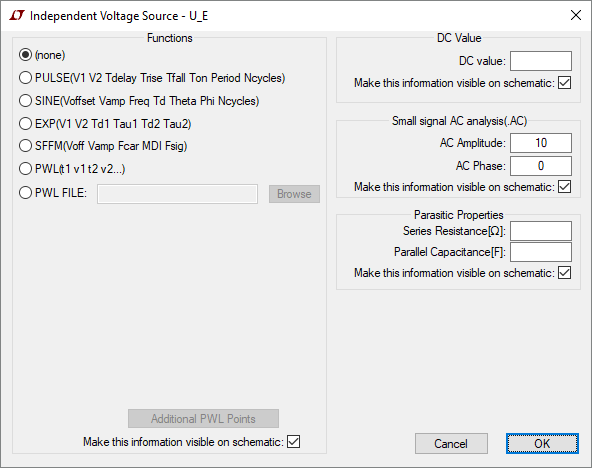
\includegraphics[width=0.9\linewidth]{src/3_Sim_Spannungsquelle.png}
  \caption{Simulation: Einstellwerte der Spannungsquelle}
  \label{fig:3_Sim_Spannungsquelle}
\end{figure}
\par
Die resultierende Simulationsschaltung ist in Abb. \ref{fig:3_Sim_Schaltung} dargestellt. Darin befindet sich neben den passiven Bauelementen und der Spannungsquelle auch ein Masse-Element zur Festlegung des Bezugspotentials. Messgeräte zur Erfassung der gewünschten Zustandsgrößen müssen in LTspice nicht gesondert eingefügt werden; die Simulation umfasst immer alle vorhandenen Zustandsgrößen.
%
\begin{figure}[H]
  \centering
  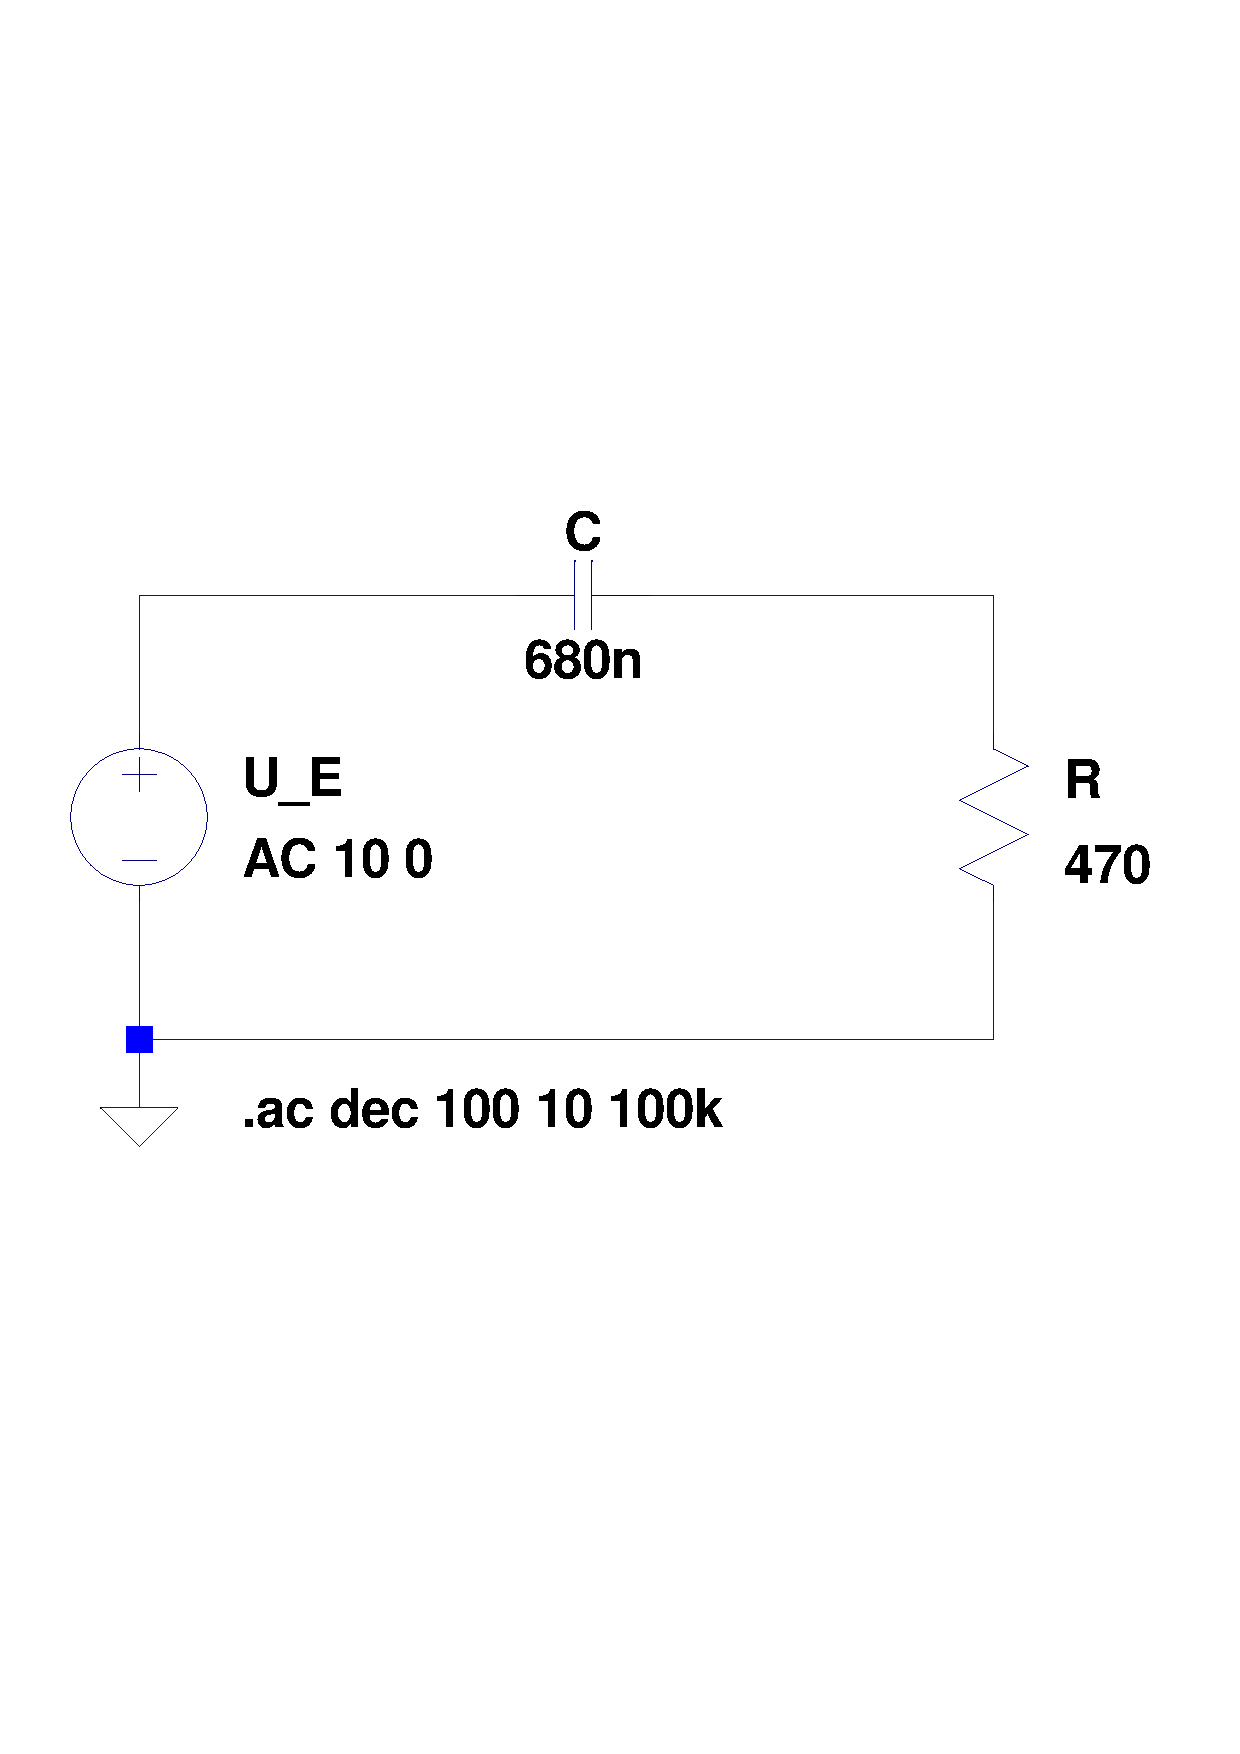
\includegraphics[width=0.6\linewidth]{src/3_Sim_Schaltung.pdf}
  \caption{Simulation: Schaltung in LTspice}
  \label{fig:3_Sim_Schaltung}
\end{figure}
%
Im Rahmen der Simulation konnte die Frequenz der Eingangsspannung über einen großen Wertebereich mit sehr vielen Stützwerten verändert werden. Während die Frequenz im Versuch zwischen $\SI{100}{\hertz}$ und $\SI{1}{\kilo\hertz}$ variiert wurde~--~bei insgesamt 10 Stützstellen~--, wurden für die Simulation Frequenzen von $\SI{10}{\hertz}$ bis $\SI{100}{\kilo\hertz}$ mit 100 Stützstellen pro Dekade verwendet. Die entsprechenden Einstellungen sind Abb. \ref{fig:3_Sim_Parameter} zu entnehmen.
%
\begin{figure}[H]
  \centering
  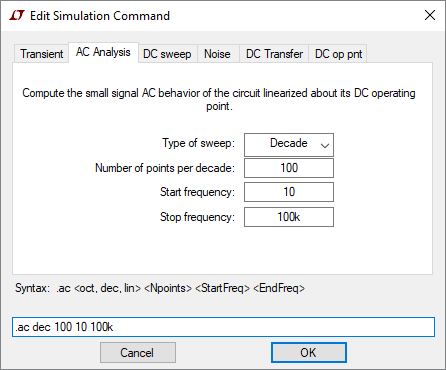
\includegraphics[width=0.7\linewidth]{src/3_Sim_Parameter.png}
  \caption{Simulation: Einstellwerte der Simulationsparameter}
  \label{fig:3_Sim_Parameter}
\end{figure}
%
Im Anschluss an die Simulation wurden die Ergebnisse aus LTspice exportiert und mit Hilfe der readLTspice-Funktion\footnote{siehe \cite{src:readLTspice}} in Scilab\footnote{siehe \cite{src:Scilab}} eingelesen. Dort wurden die Daten ausgewertet.
%
%
%